\chapter{Methodology and Experimental Setup}
\label{chap3}
% \thispagestyle{fancy}
\textit{This chapter motivates the methodologies to address the research questions while incorporating engineering subject matter, such as models, hardware platforms, and software environments pertinent to this degree project.} 

\section{Methodologies}
Concerning \hyperref[rq1]{research question 1}, the state space restriction methods discussed should be confident to restrict the state space and increase the learning efficiency, since the algorithm is constructed directly from the state space, but the effectiveness of the surrogate model is undetermined. Therefore, an assessment of the effectiveness of the surrogate model is required, taking into account key metrics such as the Root Mean Squared Error (RMSE) of prediction on the gaits, Coefficient of determination ($R^2$) between simulations and predictions on the reference, and Normalized Root Mean Squared Error (NRMSE) of observations from the sensors on the robot. Then, the independent variables that will be used are settings of parameterization parameters, rotational angle $\alpha_r$, bending angle $\alpha_b$ and compressed length of the actuator $z_l$, which was determined by previous parameterization on the continuum actuators\cite{jiOmnidirectionalWalkingQuadruped2022}. Thus, dependent variables are simulation time, prediction accuracy and long-term prediction accuracy, where long-term prediction 
\begin{itemize}
    \item Independent variables: 
    \begin{itemize}
        \item Compressed length of the actuator limit($z_l$), Type: Continuous, Units: Millimeters
        \item Bending angle limit ($\alpha_b$), Type: Continuous, Units: Radian
    \end{itemize}
    \item Dependent variables:
    \begin{itemize}
        \item Model accuracy, Type: Continuous, Units: RMSE, $R^2$, NRMSE, Percentage
        \item Long-term prediction accuracy, Type: Continuous, Units: Percentage
        \item Simulation time without failure, Type: Continuous, Units: Second
    \end{itemize}
\end{itemize}

After the data was collected, the data should be preprocess to conduct a correlation analysis to determine if there is a linear relationship between the independent variables and the dependent variable. To analyze the data, three multiple linear regressions will be conducted, with the three parameters as independent variables and each of performance metrics as the dependent variable. In addition, a best performane model should be determined from this test and proceed it to answer research question 2.
Regarding to \hyperref[rq2]{research question 2}, another ANOVA test could be conducted to evaluate the performance of model-based RL agent in comparison to model-free RL agent in terms of stability, walking speed and cost-of-transport. Firstly, the independent variables are defined as the desired walking speed and the type of RL method, with two levels: model-based RL and model-free RL. The dependent variables will be stability, walking speed, and cost of transport, measured as performance metrics during the gait. The stability of robot could be quantified by the zero-moment point (ZMP) method, while walking speed and cost-of-transport are direct performance metrics during gait. Data will be collected by simulating the gait controller using both RL methods, and measuring the three performance metrics for each simulation run, resulting in three data sets for each RL method. 
\begin{itemize}
    \item Independent variables: 
    \begin{itemize}
        \item Type of RL method, Type: Categorical, Units: Model-based, Model-free
    \end{itemize}
    \item Covariance:
    \begin{itemize}
        \item Desired walking speed ($v_x$), Type: Continuous, Units: Meter per second
    \end{itemize}
    \item Dependent variables:
    \begin{itemize}
        \item Stability, Type: Continuous, Units: Sum of moment, Newton*meter
        \item Resultant walking speed, Type: Continuous, Units: Meter per second
        \item Cost-of-transport, Type: Continuous, Units: Percentage
        \item Learning efficiency, Type: Continuous, Units: Number of iterations to converge
        \item Long-term planning , Type: Continuous, Units: Cumulative reward
    \end{itemize}
\end{itemize}
A one-way ANCOVA test will be conducted with \ac{RL} method type as one factor, and the desired walking speed as a covariance. The null hypothesis is that there is significant difference in the means of the performance metrics between the two RL methods with different desired walking speed. If the null hypothesis is rejected, it indicates that there is a significant difference in at least one of the performance metrics between the two RL methods. The test bed is listed in Table \ref{tab:rq2test}. Furthermore, a Pareto analysis will be employed to evaluate the trade-off between multiple objectives, focusing on simulation benefits, where learning efficiency can be measured by the number of iterations or episodes required for the model-based RL algorithm to converge to a satisfactory policy, long-term planning effectiveness could be measured by evaluating cumulative reward obtained by the policy over a longer horizon. The Pareto front is then determined by identifying the set of solutions that cannot be improved in one objective without worsening at least one other objective. The Pareto set can be also computed, which is the set of algorithms that correspond to the Pareto front, and the Pareto optimal solutions will also be determined, which are the objective values associated with each point on the Pareto front. 
\begin{longtable}{|p{1cm}|cccccccc|}
\hline
    \multicolumn{1}{|c|}{\multirow{2}{*}{Method}} &
      \multicolumn{8}{c|}{\begin{tabular}[c]{@{}c@{}}Desired walking\\  speed $v_x$ (m/s)\end{tabular}} \\ \cline{2-9} 
    \multicolumn{1}{|c|}{} &
      \multicolumn{1}{c|}{0.01} &
      \multicolumn{1}{c|}{0.1} &
      \multicolumn{1}{c|}{0.3} &
      \multicolumn{1}{c|}{0.5} &
      \multicolumn{1}{c|}{0.75} &
      \multicolumn{1}{c|}{1} &
      \multicolumn{1}{c|}{1.5} &
      3 \\ \hline
    \endfirsthead
    %
    \endhead
    %
    Model-based RL &
      \multicolumn{1}{c|}{\begin{tabular}[c]{@{}c@{}}Test 1:\\ Test 2:\\ Test 3:\end{tabular}} &
      \multicolumn{1}{c|}{\begin{tabular}[c]{@{}c@{}}Test 1:\\ Test 2:\\ Test 3:\end{tabular}} &
      \multicolumn{1}{c|}{\begin{tabular}[c]{@{}c@{}}Test 1:\\ Test 2:\\ Test 3:\end{tabular}} &
      \multicolumn{1}{c|}{\begin{tabular}[c]{@{}c@{}}Test 1:\\ Test 2:\\ Test 3:\end{tabular}} &
      \multicolumn{1}{c|}{\begin{tabular}[c]{@{}c@{}}Test 1:\\ Test 2:\\ Test 3:\end{tabular}} &
      \multicolumn{1}{c|}{\begin{tabular}[c]{@{}c@{}}Test 1:\\ Test 2:\\ Test 3:\end{tabular}} &
      \multicolumn{1}{c|}{\begin{tabular}[c]{@{}c@{}}Test 1:\\ Test 2:\\ Test 3:\end{tabular}} &
      \begin{tabular}[c]{@{}c@{}}Test 1:\\ Test 2:\\ Test 3:\end{tabular} \\ \hline
    Model-free RL &
      \multicolumn{1}{c|}{\begin{tabular}[c]{@{}c@{}}Test 1:\\ Test 2:\\ Test 3:\end{tabular}} &
      \multicolumn{1}{c|}{\begin{tabular}[c]{@{}c@{}}Test 1:\\ Test 2:\\ Test 3:\end{tabular}} &
      \multicolumn{1}{c|}{\begin{tabular}[c]{@{}c@{}}Test 1:\\ Test 2:\\ Test 3:\end{tabular}} &
      \multicolumn{1}{c|}{\begin{tabular}[c]{@{}c@{}}Test 1:\\ Test 2:\\ Test 3:\end{tabular}} &
      \multicolumn{1}{c|}{\begin{tabular}[c]{@{}c@{}}Test 1:\\ Test 2:\\ Test 3:\end{tabular}} &
      \multicolumn{1}{c|}{\begin{tabular}[c]{@{}c@{}}Test 1:\\ Test 2:\\ Test 3:\end{tabular}} &
      \multicolumn{1}{c|}{\begin{tabular}[c]{@{}c@{}}Test 1:\\ Test 2:\\ Test 3:\end{tabular}} &
      \begin{tabular}[c]{@{}c@{}}Test 1:\\ Test 2:\\ Test 3:\end{tabular} \\ \hline
    
    
      \caption{ANCOVA tests examples for research question 2}
      \label{tab:rq2test}
\end{longtable}

\section{Modelling}
The process of modeling a robot is a fundamental step in developing an effective controller. Modeling soft-legged robots with soft actuators is challenging due to the non-linearity, time-variant properties, and unpredictable behaviors of soft materials. Despite these difficulties, research groups from KTH Royal Institute of Technology\cite{jiSynthesizingOptimalGait2022,daneliaStructureGaitOptimizationof2021,thorapallimuralidharanContinuumActuatorBased2020,jiLearningbasedControl4D2022} have successfully constructed a soft quadruped robot using soft continuum actuators, enabling it to walk. However, the robot's movement is not yet optimal, emphasizing the necessity for continued research and development in this field. This thesis work was based on this complete soft quadruped robot model, SoftQ. 

\subsection{Physical Model}
SoftQ is a tendon-driven and lightweight robot that uses soft continuum actuators to enable it to move in a manner similar to that of a real quadruped animal. The robot's body is made up of a hollow lightweight panel, which is holding of four arrays of servo motors that are grouped and arranged to control each leg. The central board and STM32.
\begin{figure}[htb]
    \centering
    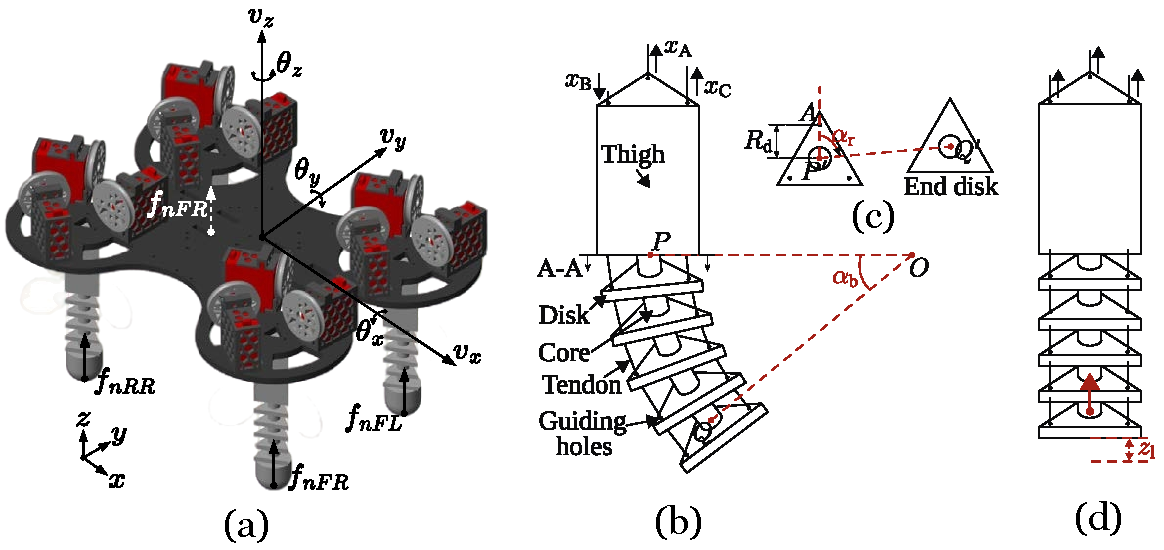
\includegraphics[width=\linewidth]{img/chap3/robots.pdf}
    \caption{Graphical overview of SoftQ and the Compressible Tendon-driven Soft Actuator (CTSA) to drive the robot. (a) Rendered robot with key state notations. (b) The structure and notations of the CTSA. The upper part from section A-A is the rigid thigh for maintaining the actuator length and the lower part is compressible and bendable. The bending angle of the lower part is noted as $\alpha_b$. (c) The top view of the bent CTSA of section A-A. $\alpha_r$ refers to the rotational angle of the CTSA. (d) The CTSA compression is realized by pulling the three tendons by the same amount, with the compression length being noted as $z_l$, originated from Ji et al.\cite{jiSynthesizingOptimalGait2022, jiOmnidirectionalWalkingQuadruped2022}}
    \label{fig:robot}
\end{figure}
\subsubsection{Actuator}
Soft continuum actuators are a type of soft actuator that can produce a continuous bending or twisting motion along the length of the actuator, without the need for discrete joints or segments. In the previous work\cite{muralidharanSoftQuadrupedRobot2021}, the it is presented the design and fabrication of a quadruped robot enabled by four CTSAs as shown in Fig. \ref{fig:robot}. Each actuator is driven by three servo motors to enable omnidirectional bending motions.

The robot design is a sophisticated design for this project, and only part of sensors will be used to guide the optimal gait controller design. The servo motor used is TS-411MG from TrackStar, which receives \ac{PWM} signals and rotates the shaft proportionally using the built-in position controller.  With all subsystems modeled, the quadruped robot system is assembled and simulated in the MATLAB Simscape environment. In this study, to enable enough bending of the actuator while still maintaining the balance of the entire robot, the maximum rotational angle of the servo motor is set as $\bar{a}_M = \pi/6$, meaning that the rotational range of the servo motor is as [-$\bar{a}_M$,$\bar{a}_M$]. The corresponding \ac{PWM} signal range is [6.67\%, 8.33\%]. The tendon-driven continuum actuator is composed of a sequential combination of rigid disks and flexible cores. The three driven tendons are equally distributed at a radial formation around the rigid disks of the actuator and passed through respective guiding holes placed on the rigid disks. Furthermore, the length of the actuators with core and disk structure is also reduced and the upper thigh is printed as solid to offer more rigidity. To model the above soft actuator deformations, the following two methods can be applied: Use lumped parameter method, where rigid components are applied to build the shape of the cores and the disks while using spring and damper joints for modeling the connections between the cores and disks and enabling the target bending and compression actuator motions. These joints use equivalent stiffness and damping to provide equal response of the entire actuator compared with the flexible segments, only needs to estimate the rigid connecting joint motions with stiffness $k$ and damping $d$ properties in the bending and longitude directions, denoted as $k_B$, $d_B$, $k_L$ and $d_L$ respectively. The tendons pass through the guide holes in the rigid disks, which allow tendon motion while holding them in place. The tendons can be simulated using the cable functions in most simulations tools, where the continuum actuators are then created in the MATLAB Simscape Multibody environment by the rigid components with telescope joints and no pulley. The contact between the feet of the quadruped robot and the ground is represented using the static and dynamic friction coefficients $f_s=0.315$ and $f_d=0.3$. The local coordinate system of the robot is defined using the right hand rule, with the front direction as the $x$ direction and the anti-gravity direction as the $z$ direction. Ten key parameters are drawn from the simulation model to represent the robot states. The roll, pitch and yaw movements are represented using the rotational angles of the body center in the three axes $x$, $y$ and $z$, noted as $\theta_x$, $\theta_y$ and $\theta_z$. The translational moving velocities are also represented by the movement of the body center in the three directions and are noted as $v_x$, $v_y$ and $v_z$, respectively. The update period of the RL algorithm is $T_s$ = 0.05s and the simulation model of the soft robot is a continuous-time model. To prevent the robot from falling down or entering unstable states in which the simulation results would be unreliable, termination boundaries are set in the simulation environment. When the robot states meet these termination conditions, the simulation ends before the desired simulation time. The roll and pitch angles of the body center $\theta_x$ and $\theta_y$, are set to rotate less than 0.15 rad, while the bending angle $alph_b$ of all the four legs are set to less than $\pi/3$.

The servo motor that receives \ac{PWM} signals and generates rotational torque via its shaft, which is then transmitted to the following subsystems. It is assumed that the rotational angle of the servo motor follows the input \ac{PWM} signals without error. The spool that is connected to the shaft of the servo motor converts the motor torque to the force in the tendon. The two ends of the tendon are connected to the spool and the end disk of the following continuum structure. When the spool rotates, the rotational motion of the spool also causes a corresponding length change of the tendon. The middle position 0 of the spool is considered as the neutral position, where the actuator is in its straight shape. When the spool angle rotates to positive values, the tendon is pulled up. For negative values, the tendon turns into slack mode. The tendon force is applied on the actuator and causes deformation. The force balance between the tendon force and reaction force of the actuator determines the deformation dynamics. Three of the motor and spool systems apply forces at equally distributed radial locations of the actuator and can lead to omnidirectional bending motion. The morphing of the actuators is realized by the traction force exerted via the tendons. Four of the above actuator systems are assembled together as the four legs of the quadruped robot. The robot is placed on the ground with gravitational forces in the simulation environment. The different motions of the four legs cause relative motion with the ground and generate static or dynamic friction, which then lead to the robot’s movement. Different ground conditions have different frictional properties and can result in different motions.
\subsubsection{Sensor}

\ac{FR}, \ac{FL}, \ac{RR}, \ac{RL2} legs 

\ac{IMU} Quaternion to represent the motion, Quaternions are a mathematical construct that extends the notion of complex numbers to four dimensions. They consist of four components, namely the scalar part, denoted by $w$, and the vector part, denoted by $\vec{v}=(x, y, z)$, and can be expressed as:
$$q = w + xi + yj + zk$$
where $x$, $y$, $z$, and $w$ are real numbers, and $i$, $j$, and $k$ are three imaginary units that satisfy the following multiplication rules: $i^2 = j^2 = k^2 = ijk = -1$. This approach entails defining the initial pose of the robot as a quaternion and obtaining the current pose using sensors such as accelerometers and gyroscopes. The change in pose between the initial and current poses is then calculated, and the rotational component is extracted. From the rotational component, the rotation axis and angle can be determined. The velocity of the robot can be obtained by differentiating the position component of the current pose with respect to time. The velocity vector is then transformed into the world coordinate frame using the current orientation of the robot. The angular velocity vector and the linear velocity vector are the final output of the calculation.
Force sensors 
\ac{ToF} sensor 
Optical camera

\subsubsection{flexible structure deformation system}





\subsection{Modeling in MathWorks Simulink\texorpdfstring{\textsuperscript{\textregistered}}{(R)}}
The model of this quadruped robot comprises several subsystems, including the motor-driven units, the tendon transmission mechanism, the flexible structure deformation system, and the ground contact subsystem. 

In addition, because of the influence of external gravity, the force required to move the motor at the same angle is different for different leg suspension positions, so the leg model of the quadruped is nonlinear, so that it is common to use a model predictive controller for rigid quadruped robots. However, it is not easy to predict the behavior of a soft robot if using a model predictive controller\cite{bemporadLinearTimevaryingNonlinear2022}, so it is desired to have more identical solutions for the controllers, whereby the  reinforcement learning came to our mind\cite{hewingLearningbasedModelPredictive2020}. Typically, the loads of rigid legs are different between the two cases of leg suspension and stepping on the ground\cite{biswalDevelopmentQuadrupedWalking2021}, which means that the dynamics of the quadruped robot is a mixture of continuous and discrete, such that the model is continuous when touching the ground or when hovering, but there is a sudden change from hovering to touching the ground, which makes the model behave a discrete. 

Additionally, applying \ac{RL} to train the gait controller involves creating a virtual model of the robot and its environment to simulate possible walking behaviors and test the efficacy of various control policies. This approach is motivated by the challenges associated with collecting data in the physical world, which can be time-consuming, costly, and hazardous. By leveraging the benefits of simulation, the training process can generate a large volume of data quickly and inexpensively, allowing for the exploration of a broad range of behaviors and control policies without exposing the physical robot to potential risks. This methodology facilitates the application of deep learning and reinforcement learning techniques to develop a robust and efficient gait controller for the soft quadruped robot. The simulation-based approach allows for efficient iteration and optimization of the training process, resulting in a control policy that can be effectively applied to the physical robot.

\section{Surrogate Model}

\subsection{Neural Networks}

Applying engineering related and scientific skills; modelling, analysing, developing, and evaluating engineering-related and scientific content; correct choice of methods based on problem formulation; consciousness of aspects relating to society and ethics (if applicable).

\section{Experiment Setup}

\begin{table}[ht]
    \centering
    \begin{tabular}{ll}
        \toprule
        Component        & Description                             \\\midrule
        Operating System & Windows 10                              \\
        \ac{IDE}              & MATLAB R2021b                           \\
        \ac{CPU}              & Intel(R) Core(TM) i7-4770 CPU @ 3.40GHz \\
        Memory           & 16 GB                                   \\\bottomrule
        \end{tabular}%
    \caption{Development environment for stochastic model}
    \label{tab:env}
\end{table}



As mentioned earlier, give a theoretical description of methodologies and methods and how these are applied in the degree project.
Boxes can be used to organize content
\begin{tcolorbox}[title={Development environment for stochastic model}]
	\tt{
		\textbf{Operating systems }\\
		computer: Linux - kernel 4.18.5-arch1-1-ARCH\\
		android phone: 8.1.0\\
		~\\
		\textbf{Build tools}\\
		exp (build tool): version 55.0.4\\
		~\\
		...
	}
\end{tcolorbox}
